%----------------------------------------------------------------------------------------
%
% Master's Thesis Project Proposal, 5DV50E
% By: Prasannjeet Singh, ps222vt@student.lnu.se
% Department of Computer Science
% Linnaeus University
%
%----------------------------------------------------------------------------------------

%----------------------------------------------------------------------------------------
%	The Preamble
%----------------------------------------------------------------------------------------
\documentclass[a4paper,10pt,table,xcdraw]{thesis}
\usepackage[english]{babel}
\usepackage[utf8]{inputenc}
\usepackage{wallpaper}
\usepackage[absolute]{textpos}
\usepackage[top=2cm, bottom=2.5cm, left=3cm, right=3cm]{geometry}
\usepackage{xltxtra} % Using this for loading custom text font
\usepackage[font=footnotesize,labelfont=bf]{caption} %for smaller size of caption
\usepackage{wrapfig} % for wrapping figure left or right
\usepackage[style=ieee, backend=biber]{biblatex} %for bibliography
\usepackage{framed} %for adding a framebox
\usepackage[framemethod=tikz]{mdframed} %to change the background color in 'begin{framed}
\usepackage{listings} % for \listingputlisting
\usepackage{tabto} %for using tabs
\usepackage{caption} %because for some reason, caption for figure 1.1 does not show traditioanlly
%\usepackage[hang,flushmargin]{footmisc}  % for left indenting footnotes
\usepackage{scrextend} %for footnote indentation (using \deffootnote)
\usepackage{hyperref} %for adding hyperlinks to citations and references
\usepackage{xcolor}
%\usepackage[]{xcolor} %for defining colors of hyperlinks in \hypersetup{}
\usepackage{enumitem} %for customising bullet point format (in RQ1, RQ2, etc.)
\usepackage{booktabs} %for using tables in the section time plan
\usepackage{tabularx} %for auto fitting the tables

%----------------------------------------------------------------------------------------
%	Other Settings
%----------------------------------------------------------------------------------------
\tolerance=1					%prevent hyphenating
\emergencystretch=\maxdimen		%prevent hyphenating
\hyphenpenalty=10000			%prevent hyphenating
\hbadness=10000					%prevent hyphenating
\addbibresource{references.bib} %for bibliography
\author{Prasannjeet Singh}
\renewcommand{\footnotesize}{\scriptsize} %decreasing the footnote size
\deffootnote{2em}{0em}{\thefootnotemark\quad} %for formatting footnote labels
\hypersetup{		% defining hyperlink colors
	colorlinks,
	linkcolor={red!50!black},
	citecolor={blue!80!black},
	urlcolor={blue!50!black},
	hyperfootnotes
}
\def\changemargin#1#2{\list{}{\rightmargin#2\leftmargin#1}\item[]} 	%for paragraphs with...
\let\endchangemargin=\endlist 										%different margin

%----------------------------------------------------------------------------------------
%	Title section
%----------------------------------------------------------------------------------------

\newsavebox{\mybox}
\newlength{\mydepth}
\newlength{\myheight}

\newenvironment{sidebar}%
{\begin{lrbox}{\mybox}\begin{minipage}{\textwidth}}%
		{\end{minipage}\end{lrbox}%
	\settodepth{\mydepth}{\usebox{\mybox}}%
	\settoheight{\myheight}{\usebox{\mybox}}%
	\addtolength{\myheight}{\mydepth}%
	\noindent\makebox[0pt]{\hspace{-20pt}\rule[-\mydepth]{1pt}{\myheight}}%
	\usebox{\mybox}}

\newcommand\BackgroundPic{
	\put(-2,-3){
		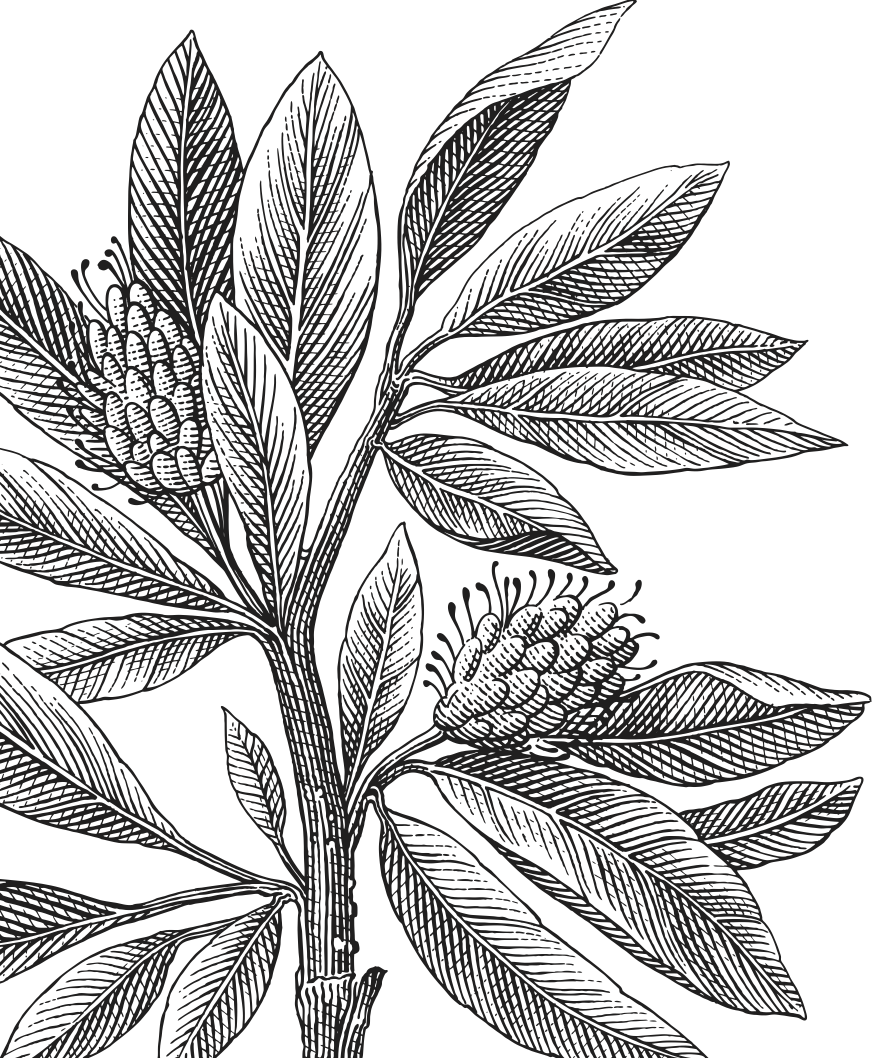
\includegraphics[keepaspectratio,scale=0.3]{images/lnu_etch.png} % Background picture
	}
}
\newcommand\BackgroundPicLogo{
	\put(30,740){
		
\includegraphics[keepaspectratio,scale=0.10]{images/logo.png} % Logo in upper left corner
	}
}

\title{	
	\vspace{-8cm}
	\begin{sidebar}
		\vspace{10cm}
		\normalfont \normalsize
		\Huge Master's Degree Project Proposal \\
		\vspace{-1.3cm}
	\end{sidebar}
	\vspace{3cm}
	\begin{flushleft}
		\huge Distributed Information Flow Control in Android Applications\\ 
%		\it \LARGE - Optional subtitle 
	\end{flushleft}
	\null
	\vfill
	\begin{textblock}{6}(9,13)
		\begin{flushright}
			\begin{minipage}{\textwidth}
				\begin{flushleft} \large
					\emph{Author:} Prasannjeet Singh\\ % Author
					\emph{Supervisor:} Narges Khakpour\\ % Supervisor
					%\emph{Examiner:} Dr.~Mark \textsc{Brown}\\ % Examiner (course manager)
					\emph{Course Code:} 5DV50E\\
					\emph{Semester:} HT 2021\\ % 
					\emph{Department:} Computer Science\\ % Subject area
				\end{flushleft}
			\end{minipage}
		\end{flushright}
	\end{textblock}
}

\date{} 

\begin{document}
	\pagenumbering{gobble}	
	\newgeometry{left=5cm}
	\AddToShipoutPicture*{\BackgroundPic}
	\AddToShipoutPicture*{\BackgroundPicLogo}
	\maketitle
	\restoregeometry
	\clearpage
	\selectlanguage{english}
	
%----------------------------------------------------------------------------------------
%	Table of Contents
%----------------------------------------------------------------------------------------
	\renewcommand*\contentsname{Table of Contents}
	\tableofcontents % Table of contents
	\newpage
	\pagenumbering{arabic}
	
%----------------------------------------------------------------------------------------
%	Setting main font for the rest of the document
%----------------------------------------------------------------------------------------
	\setmainfont[
	BoldFont={Charter Bold}, 
	ItalicFont={Charter Italic},
	]{Charter}
%----------------------------------------------------------------------------------------
%	All Other Sections
%----------------------------------------------------------------------------------------
	
	\chapter{Background}
	In this document, we propose to construct an approach to secure a serverless system using \textit{Distributed Information Flow Control}. For a system to be secure at the programming level, it is imperative that \textbf{confidentiality} and \textbf{integrity} is enforced. While confidentiality is described as the virtue of a system to protect it's sensitive data from being disclosed to unauthorized parties, where as integrity can be explained as the ability of a system to prevent an information from being manipulated or modified by unauthorized parties. Going forward, all the essential ideas will be elaborated in this section as follows: \ref{section:ServerlessComputing} introduces \textit{Serverless Computing}, where as \ref{section:InformationFlowControl} talks about the information flow control model. Furthermore, \ref{section:NonInterference} describes the security property of \textit{non-interference} in security, and \ref{section:TSNI} describes two types of information flow control enforcements, \textit{Termination Insensitive Non Interference} (TINI), and \textit{Termination Sensitive Non Interference} (TSNI). Here, TSNI is described formally. Finally, \ref{section:ExistingApproaches} discusses existing approaches that employ IFC to secure serverless systems.

\section{Serverless Computing}
\label{section:ServerlessComputing}
With the rise in usage of Cloud Computing, different architectures have been introduced by vendors over time, increasing efficiency, performance, and at the same time, decreasing the cost. In the early days, Infrastructure as a Service, or IaaS was prevalent, which provided virtual servers in the cloud. However they were still servers, with the difference being - the need to personally own the servers was not required anymore. Further, the concept of PaaS, or Platform as a Service was introduced, that delivered virtual application platforms, viz. JAVA Spring Boot, Python Flask, Node JS Express, etc. Here, the developers were no more responsible for maintaining the operating system. Nevertheless, packaging an application for deployment and  managing the scalability was still critical. Although after the introduction of container orchestration platforms such as Docker Swarm, Kubernets, etc. PaaS has started gaining more popularity.
%\footnote{B. Christner, “Docker Serverless,” 2017. [Online]. Available:
%	https://pt.slideshare.net/BrianChristner/docker-serverless?from\_action=save}


%\begin{wrapfigure}{r}{0.71\textwidth} %this figure will be at the right
	\begin{framed}
		\centering
		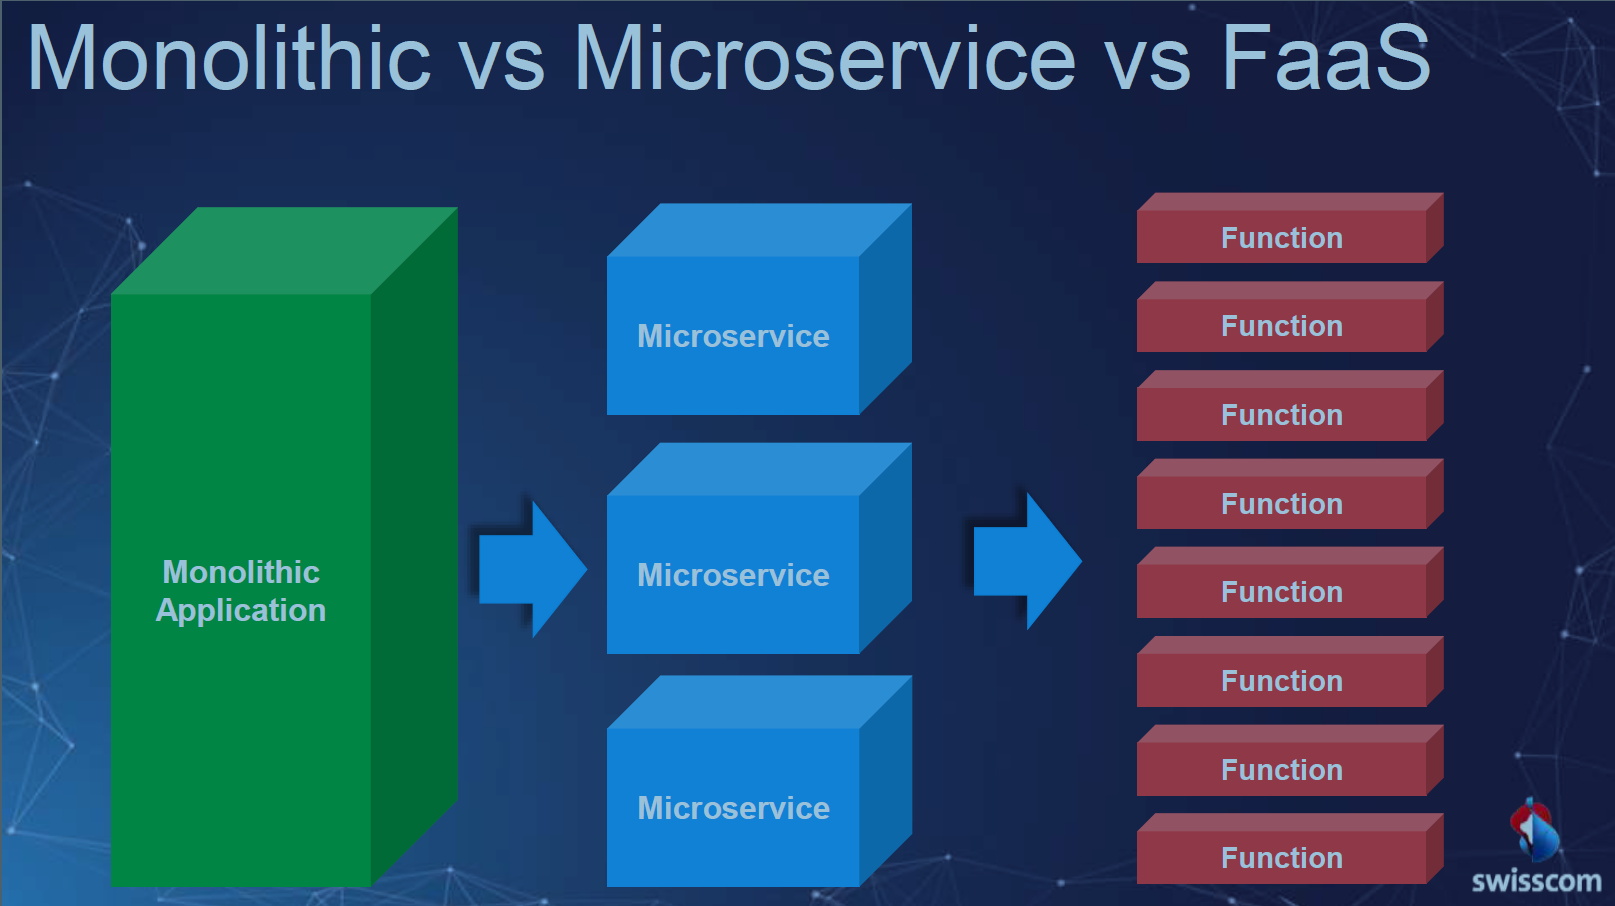
\includegraphics[width=\textwidth]{images/monoVSmicroVSfaas.png}
		\captionof{figure}{Graphical representation of the architectural difference between a Monolithic Application (IaaS), a Microservices-Based Application (PaaS), and Serverless (FaaS)
		}
		\label{fig:IaaSPaaSFaaS}
	\end{framed}
%\end{wrapfigure}


Finally, Functions as a Service (FaaS), or \textit{Serverless Computing} was introduced, which can intuitively be perceived as taking the resource abstraction to its logical \mbox{conclusion \footnotemark}. \addtocounter{footnote}{0} \footnotetext{S. Waterworth, “Introduction to Serverless Computing,” 2018.
https://www.instana.com/blog/introduction-to-serverless-computing/} It is needless to say that Serverless Computing still involves servers. However in this case, developers spend minimum time in maintaining or managing servers as compared to previous-generation architectures. Instead of accommodating a monolith application or a collection of microservices, Serverless architecture only contains a set of functions deployed individually. Figure~\ref{fig:IaaSPaaSFaaS} shows the contrast between the aforementioned architectures\footnote{B. Christner, “Docker Serverless,” 2017. https://pt.slideshare.net/BrianChristner/docker-serverless}.

\section{Information Flow Control}
\label{section:InformationFlowControl}
Information flow control, or IFC mainly focuses on building secure systems irrespective of the fact that the system might contain faults or bugs. It is difficult to build secure systems in the first place, as a single bug in any line of code may lead to security vulnerability. Therefore, it is not surprising to learn that in many cases, a simple bug has resulted in the disclosure of many sensitive information, such as personal identity, credit card numbers, etc.\footnote{L. H. Newman, “The Equifax Breach Was Entirely Preventable,” Wired, 2017. https://www.wired.com/story/equifax-breach-no-excuse}$^{,}$\footnote{Big data breach! Aadhaar software hack raises major security concerns, BusinessToday. https://www.businesstoday.in/current/economy-politics/aadhaar-software-hack-uidai-data-ghost-entries/story/282260.html}$^{,}$\footnote{T. Armerding, “The 18 biggest data breaches of the 21st century,” CSO Online, 2018. https://www.csoonline.com/article/2130877/the-biggest-data-breaches-of-the-21st-century.html}. As a result, there are a lot of strategies available currently that focuses on finding and fixing bugs such as SQL Injection, Temporary file races, Buffer overflows, Missing access checks, Format string bugs, Integer overflow, etc. However, it is important to note that most of these bugs require different methodologies in order to tackle them; and therefore, it has eventually become a battle between the attacker and security expert for who find the next bug in a system first. In case of the former, the system might be exploited and in case of the latter, the bug might be fixed, and the system made secure – until the next bug is discovered. As it can be observed, this approach to make the system secure does not appear to be practical, as it can eventually turn out to be risky and costly, since declaring a system completely bug-free is not possible.\footnote{SteelKiwi Inc, “Is There Such a Thing As Bug-free Software?,” Hackernoon, 2018. https://hackernoon.com/is-there-such-a-thing-as-bug-free-software-320cd862af17.}$^{,}$\footnote{R. Varshneya, “There’s No Such Thing as a Bug-Free App,” Entrepreneur India, 2015. https://www.entrepreneur.com/article/251742}$^{,}$\footnote{Allen, “The Myth of ‘Bug Free’ Software,” BetaBreakers, 2016. https://www.betabreakers.com/the-myth-of-bug-free-software}

Let us contemplate a small illustration to support our argument – consider a simple eCommerce website that sells books online. The web-application is built under different layers of abstraction, as shown in the Figure~\ref{fig:eCommerceArchitecture}. The web application itself enforces some kind of security policy that restricts one user to access the credit-card or address information of any other user. Going a level down, the web server, such as Apache could have its own security policy that ensures which web browser can make what http requests, etc. Going deeper, the operating system might have some enforcements to protect different Windows/UNIX users from one another. In the same vein, the hardware could be providing some mechanism to protect the kernel from application code, etc. As we can intuit, for the whole system to be secure, the code at every abstraction layer must be correct, or bug-free. However, as we are aware, all these layers combined comprise of millions of lines worth of code, and therefore, occurrence of one or more bugs anywhere up the stack is inevitable. Consequently, it can be said that the strategy of securing a system by the means of fixing a bug is practically impossible. This implies that securing a system completely via fixing all the discovered bugs is impossible. Nevertheless, via Information Flow Control, it is indeed possible to build a secure system despite the existence of bugs in the code.

\begin{figure}[h]
	\begin{framed}
		\centering
		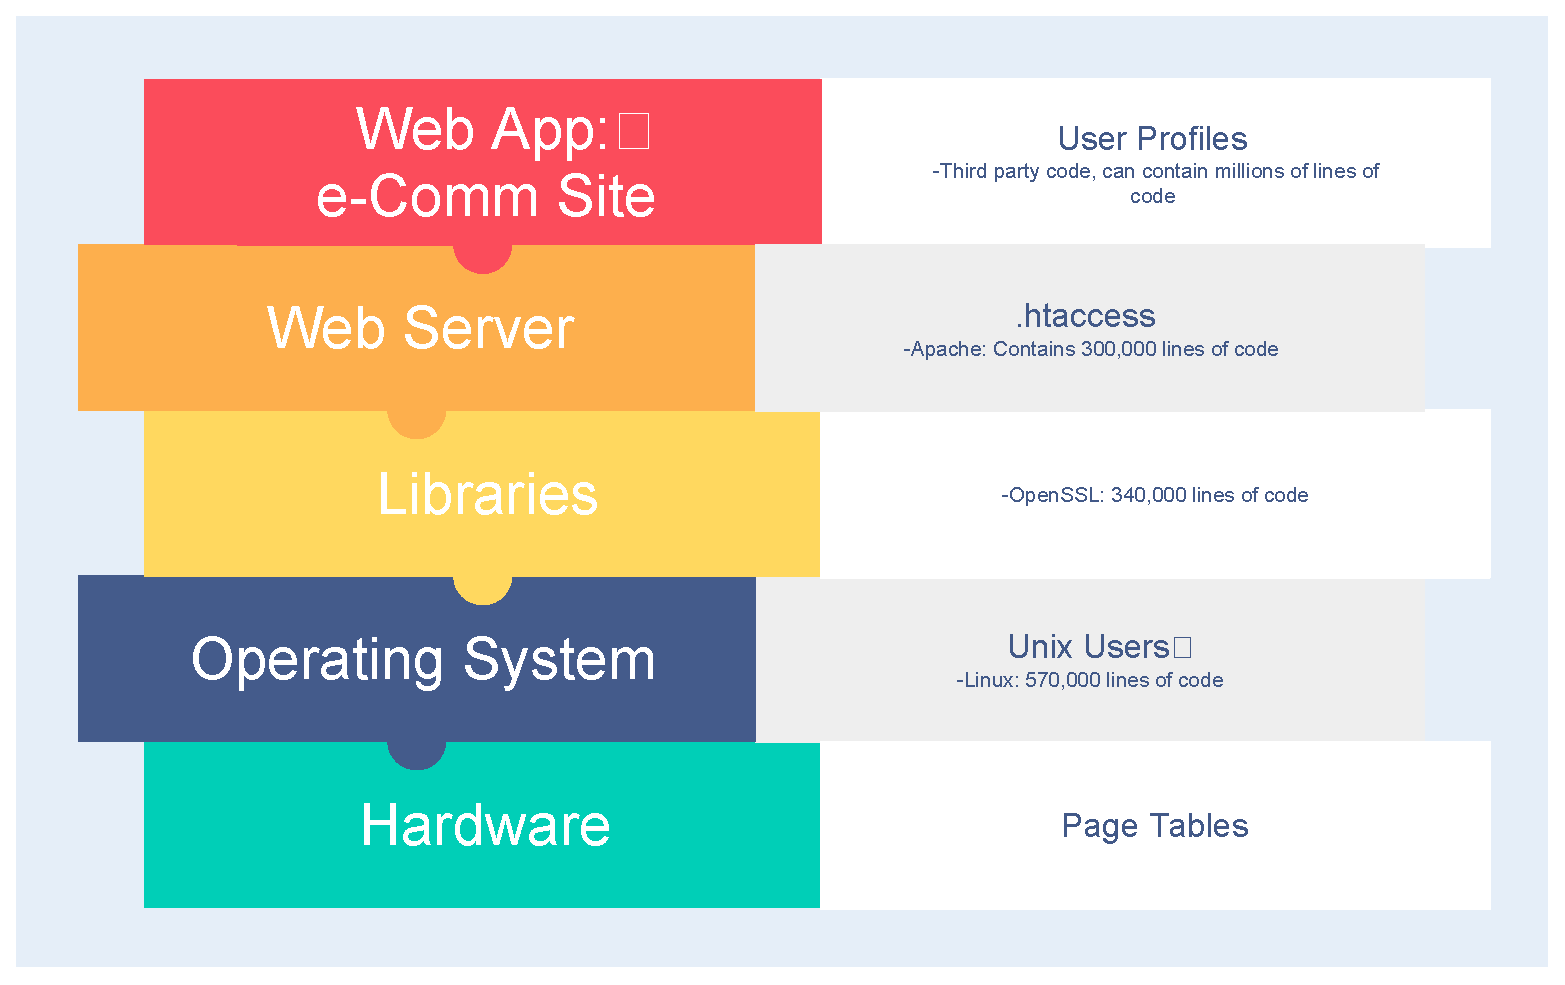
\includegraphics[width=\textwidth]{images/architectures.eps}
		\caption{A software architecture diagram for a simple e-commerce web application.}
		\label{fig:eCommerceArchitecture}
	\end{framed}
\end{figure}

Let us now take a step back and realise the fact that ensuring the security of a system is, in varying degrees, dependent on the data, rather than the code. As an instance, in the example shown in above (Figure~\ref{fig:eCommerceArchitecture}), a user wouldn’t want their credit-card data to be unauthorizedly accessed or sent to another location by an attacker. Assuming we can \textit{control and monitor all these data movements in a system}, and so long as the data remain secure, it is of no concern to supervise what is being done to the data by the application code. Trying to secure a system through this approach achieves the goal to secure the system without caring about the existing bugs in the system. Furthermore, enforcing IFC at lower abstraction level in an application ensures that the application remains secure in all the above abstraction levels. IFC is conceptually a simple idea: A label is associated with every piece of data in a system, and this label usually applies to data at all different levels of abstraction, ranging from \textit{hardware} to the \textit{application data}. Additionally, this label follows the data as it moves around through the system, and ultimately this label specifies what can happen to the data. For instance, it can make sure that the copy a user's credit-card number cannot be sent to an attacker's website. If this idea of Information Flow Control is implemented appropriately, the hope is that a system could be made secure without concerning ourselves with numerous existing bugs in the system.

The information flow model is an extension of the state machine model that constantly monitors the situation of a system to restrain it from entering an insecure state. A system that supports a state machine model must have the potential states of its process inspected in all the circumstances to confirm that they are controlled. Under the benchmarks laid down by the model, a system that boots up in a secure state and preserves the security of any transaction throughout itself shall, at all times, be in a secure state. Consequently, the information flow model consists of state transitions, objects and lattice states that regulate data flow policy. The fundamental purpose of information flow model is to restrict the flow of insecure and unauthorized data in any direction throughout the system. The exchange of data across different systems could be regulated using \textit{guards}, that can be employed by the information flow model. \textit{Flume} is a popular decentralized information flow control (DIFC)\cite{Myers2000} model and system ``\textit{that applies at the granularity of operating system processes and standard OS abstractions (e.g., pipes and file descriptors)}''\cite{Krohn2007}. 

\section{Non Interference}
\label{section:NonInterference}
Non-Interference in this research refers to the protection of the secret (\textit{high-sensitive}) part of the memory from an attacker who can observe the public (\textit{low-sensitive}) part of the memory\cite{Sabelfeld2005}. It is a policy that imposes an attacker to not be able to make a distinction between two computations from their outputs, in case they vary only in their secret inputs. It was first proposed in 1982\cite{Gougen1982}, and is a further development of the information flow model built to assure that the objects and subjects at different security level do not interfere with each other. In this context, the subjects may be applications, system users, or processes, while objects can be processes, bits of data, programs or documents. Additionally, \textit{information flow monitors} is an evolved technique that dynamically enforces noninterference. As one would expect, dynamic monitors enforce non interference differently for different instances of the execution of process under observation. This is because the information control flow of a program can be different for different input values, thus making the program secure for some set of values, while declaring it insecure for others. This is in contrast with static monitors, that will completely declare a program insecure, even if it becomes insecure for a very small range of input values. Therefore, it can be said that dynamic monitors allows analysis in further details, as compared to static monitors, as it is in the beginning of the execution of a dynamic monitor, when the assignment of security levels to the variables takes place. Moreover, the assigned security levels do not change throughout the execution. Adding to this, there also exists several \textit{hybrid} monitors \cite{Shroff2007, Russo2010, Guernic2007} that combine both static and dynamic methodologies.\par
It must, however be noted that even dynamic monitors are prone to produce false positives. Hence, there is a need to construct improved monitors that allow multiple \textit{paths}. These challenges were scoped by Khakpour and Skandylas in their research \cite{Khakpour2018} where a new approach was proposed that, at some designated checkpoints, supervises a program written in a subset of Java based on boolean supervisory controller synthesis \cite{BERTHIER201446} to construct a hybrid monitor that, to avoid future leakages, applies suitable countermeasures in checkpoints by forecasting security breaches. This approach is supported by a tool implemented in OCAML and uses SOOT to analyze the program at the java bytecode level.

\section{Termination Sensitive Non Interference}
\label{section:TSNI}
Information Flow Control (IFC) \cite{Denning1976, Hedin2011} based security techniques could be an optimistic approach to tackle the security problem in Serverless Applications. However, a security policy known as Termination Insensitive Non-Interference (TINI) have been implemented by most of the previous implementations. Intuitively, it is ensured by TINI that a program's non secret outputs are not allowed to expose any secrets stored in the system. On the other hand, the fact that the system ceased to generate outputs could be utilized to deduce some part of the secret. This channel, also known as the \textit{termination-channel} is usually neglected as it just leaks one bit. Furthermore, Askarov et al. have claimed that it might leak more than just a bit \cite{Askarov2008}. However, for Serverless Applications, even the leakage of a single bit might be dangerous, as these are highly scalable and triggering parallel computations, each leaking one bit could be performed to access the secure data. Another strong security policy, called as Termination Sensitive Non Interference (TSNI) \cite{Sabelfeld2001} could be enforced that eliminates the termination channel. Let us formally define TSNI followed by observing an example:\par
\medskip
%\begin{minipage}{\textwidth}
	\begin{mdframed}[linewidth = 0.05cm, backgroundcolor=blue!20, nobreak=true]
		\noindent Consider a Program \textbf{P}:
		\begin{framed}
			\lstinputlisting[language=Octave]{codes/tsni.txt}
		\end{framed}
		\noindent \textbf{We define some notations as:}\par
		{cH} \tab Input Channel \par \medskip
		\textbf{P} \tab The above program \par \medskip
		$\mu$ \tab Memory \par \medskip
		$State<P,\mu>$ \tab A program state. \par \medskip
		$terminating(P, \mu, I)$ \tab If the $State<P,\mu>$ is executed with input $I$, \tab \tab \tab then it terminates. \par \medskip
		$I_{1} = _{L} I_{2}$ \tab both $I_{1}$ and $I_{2}$ belong to the same security \tab \tab \tab level \textbf{L}, which can either be public or \tab \tab \tab confidential. \par \medskip
		\noindent $State<P,\mu>$ is TSNI  $\forall I_{1} \& I_{2} \iff$
		\begin{framed}
			\begin{equation} \label{eq:TSNI}
			I_{1} = _{L} I_{2} \land terminating(P, \mu, I_{1}) \Longrightarrow terminating(P, \mu, I_{2})
			\end{equation}
		\end{framed}
		\noindent \textbf{TSNI either converges or diverges $\forall$ I $\equiv$ L}
	\end{mdframed}
%\end{minipage}
\medskip
As an example, for the program \textbf{P} above, let us consider a \textbf{State} $<P, \mu>$ where two inputs $I_{1}$ \& $I_{2}$ belong to the same channel \textbf{cH} and are of the same security level, which is \textit{confidential}. Therefore, $I_{1} = _{L} I_{2}$, where \textit{L} is a \textit{confidential} security level. Let us now consider the values of $I_{1}$ \& $I_{2}$: \par
\begin{itemize}
	\item $I_{1} = [cH: 0]$
	\item $I_{2} = [cH: 1]$
\end{itemize}
It is known that in program P, an input where h>0 will result in an infinite loop, whereas any input that does not satisfy the above condition will terminate. Therefore, based on the input values assigned to $I_{1}$ \& $I_{2}$, we can say that:
\begin{equation} \label{eq:NoTSNI}
I_{1} = _{L} I_{2} \land terminating(P, \mu, I_{1}) \Longrightarrow \neg terminating(P, \mu, I_{2})
\end{equation}
As it can be clearly observed, the Equation \ref{eq:NoTSNI} above contradicts the definition of TSNI in Equation \ref{eq:TSNI} in Page \pageref{eq:TSNI}. Hence, it can be stated that the \textbf{State} $<P, \mu>$ does not satisfy TSNI.

\section{Existing Approaches}
\label{section:ExistingApproaches}
\textit{Google Scholar}\footnote{Google Scholar - https://scholar.google.co.in/}, which could be considered as one of the biggest search portal for scientific literature was used to look for other existing approaches that uses Information Flow Control to secure a Serverless system. Following were the set of keywords used:
\begin{center}
	\begin{mdframed}[frametitle=Keywords Used, linewidth = 0.05cm, backgroundcolor=blue!20, nobreak=true]
		\textit{(tsni \textbf{OR} tini \textbf{OR} "termination sensitive non interference" \textbf{OR} "termination insensitive non interference" \textbf{OR} "information flow control" \textbf{OR} "distributed information flow control" \textbf{OR} difc \textbf{OR} ifc) \textbf{AND} (serverless \textbf{OR} "serverless computing")}
	\end{mdframed}
\end{center}
Based on the above keyword-combination, we could only find one relevant research that uses Information Flow Control to secure a Serverless Computing system. This approach, proposed by Alpernas et al. \cite{Alpernas2018} aims to secure a serverless computing system by ensuring confidentiality via enforcing termination sensitive non interference (TSNI). The tool developed by the authors, called as Trapeze Framework \footnote{Trapeze Framework - https://github.com/kalevalp/trapeze} is written in JavaScript and at the moment, only supports the node.js runtime. The author claims that TSNI enforcement is essential in case of serverless computing, since the termination channel, which usually leaks just a bit cannot be disregarded; as the attacker can amplify the termination channel by executing many parallel computations, each leaking one bit.
	\newpage
	
	\chapter{Motivation}
	The functions deployed in Serverless run on-demand and webmasters are billed by the millisecond of execution time. Therefore, if the function is unused, it's \textit{free}. In this case, everything that the application needs to run is completely abstracted by the cloud platform, and in turn, it handles failover, scalability, load balancing, etc. Like other architectures, the server-side logic is still written by the application developers but in contrast, the logic here is in the form of individual functions that are run in event-triggered and ephemeral stateless compute containers and are managed by a third party completely. The containers are created on demand and destroyed as soon as the function is executed. These functionalities have catered to Serverless architecture gaining huge popularity over time (Figure~\ref{fig:ServerlessPopularity})\footnote{Google Trends, “Popularity of the keyword Serverless,” 2019. http://bit.ly/GoogleServerless}. Amazon's AWS Lambda \footnote{Amazon, “AWS Lambda – Serverless Compute - Amazon Web Services.” https://aws.amazon.com/lambda/} is currently the most popular provider of Serverless Architectures. However, other players like Google Cloud Functions \footnote{Google, “Cloud Functions - Event-driven Serverless Computing.”
	https://cloud.google.com/functions/}, Azure Functions \footnote{Microsoft, “Azure Functions—Serverless Architecture.” https://azure.microsoft.com/en-us/services/functions/}, IMB Cloud Functions \footnote{IBM, “IBM Cloud Functions.” https://console.bluemix.net/openwhisk/} and Pivotal Function Service \footnote{Pivotal Software, “Pivotal Function Service (PFS),” jan 2017.
	https://pivotal.io/platform/pivotal-function-service} have also started gaining popularity.

\begin{figure}[h]
	\begin{framed}
		\centering
		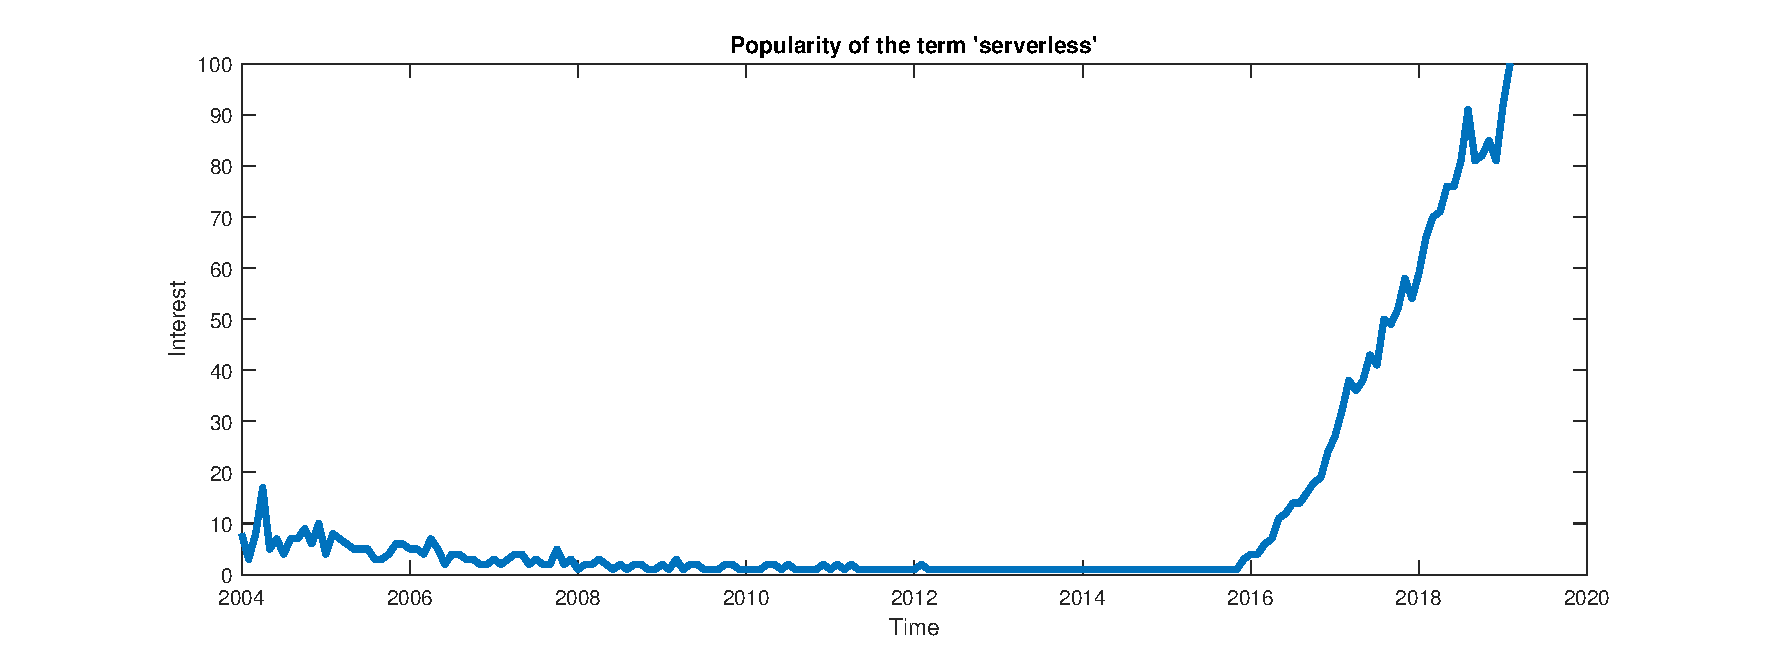
\includegraphics[width=\textwidth, trim={2.45cm 0 2.45cm 0},clip]{images/serverless_popularity.eps}
		\caption{A trends graph from Google showing the search interest of the term \textit{serverless} over the past fifteen years. Numbers represent search interest relative to the highest point on the chart for the given region and time. A value of 100 is the peak popularity for the term. A value of 50 means that the term is half as popular.}
		\label{fig:ServerlessPopularity}
		
	\end{framed}
\end{figure}

With the benefit of pay-per-use, zero-administration, ease of deployment and auto-scaling, Serverless also comes with new vulnerabilities. It does not have adequate security testing, as testing a serverless application can be far more complex than standard applications. As a result, many scanning tools haven't yet adapted to Serverless applications. Secondly, the application has an increased attack surface, as it consumes data from many event sources, namely cloud storage, HTTP APIs, IoT device communications, message queues, etc. A report from Puresec \cite{Segal2018} describes in detail the ten most critical security risks in Serverless architectures. Hence, a robust solution for the security of Serverless applications is needed.
	\newpage
	
	\chapter{Problem Statement}
	Being a fledgling technology, Serverless is yet to receive the required attention, and as a result, it is strongly vulnerable to external attacks. Furthermore, it is important to ensure Confidentiality and Integrity of data in an application. The virtue of a system to allow only authorized users the access to protected and sensitive data while shielding the data from harmful invaders is called Confidentiality. Additionally, Integrity alludes to the methodologies that ensure the authenticity of data, and the fact that it is accurate, and confidential.

IFC models have previously been implemented for traditional applications. The proposed work by Khakpour et. al \cite{Khakpour2018} works on Symbolic Confidentiality Guards Synthesizer, or SCGS, \footcite{N. Berthire and N. Khakpour, “Symbolic Confidentiality Guards Synthesizer — (SCGS),” Department of Computer Science, University of Liverpool and Department of Computer Science and Media Technology, Linnéuniversitetet, 2018. https://cgi.csc.liv.ac.uk/~nberth/scgs/.} which is a static analysis tool that primarily identifies any confidential data leak automatically in object-oriented programs. The aforementioned work supports centralized IFC where it synthesizes security guards for single methods in an application. In this work, we will extend it with decentralized IFC to enforce confidentiality and integrity in serverless computing.

 Moreover, an IFC system for Serverless Applications has also been developed \cite{Alpernas2018} as discussed previously. While the former enforces TINI for traditional JAVA applications, the latter implements the TSNI model for Serverless functions written in JavaScript for the node.js runtime. Furthermore, it only focuses on data \textit{confidentiality} and does not enforce data \textit{integrity}. Therefore a strong framework is needed for the security of Serverless Applications that enforces both data \textit{confidentiality} and \textit{integrity}. Additionally, other programming languages should also be focused upon. Based on the above discussions, we can elicit the ensuing \textbf{research questions} targeted to our study:
\begin{changemargin}{2cm}{0.5cm} 
	\begin{enumerate}[label=\textbf{RQ{{\arabic*}}:} ]
		\item
		Can an approach designed for native Java applications to enforce confidentiality and integrity be equally effective for a Java based serverless application? Why?
		\item
		What is the recommended approach to make a Java based serverless application secure, using distributed information flow control?
		\item 
		Can a tool that analyzes the Java based serverless application be built based on the aforementioned approach?
	\end{enumerate}
\end{changemargin} 
	\label{section:ProblemStatement}
	\newpage
	
	\chapter{Contributions}
	In continuation to what was discussed in the Problem Statement, an IFC modeled tool in the form of an Artifact that enforces TSNI will be fabricated that will, either statically or dynamically monitor the information flow of a Serverless JAVA program, and ascertain its security. It will be an extension to \cite{Khakpour2018} that enforces TINI and was made for native JAVA applications. Therefore, the key contributions for this thesis would be the following:
\begin{enumerate}
	\item A distributed IFC approach will be proposed for enforcing security in serverless computing that will extend the current centralized approach\cite{Khakpour2018}.
	\item Intra-behavioral analysis will be considered to check and enforce security in serverless computing.
	\item The approach will be supported by a tool built upon the current tool\cite{Khakpour2018}.
	\item The approach will be tuned to the nature of serverless computing.
\end{enumerate}
	\newpage
	
	\chapter{Approach}
	To investigate and find a solution for the problem described above, an approach of \textbf{Design Science Research (DSR)} \cite{March1995} will be followed, wherein a new artifact, in the form of a solution to the aforementioned problem will be created that will include generating new knowledge. Simon describes \textit{artifact} as an entity created by humans, rather than something occurring naturally \cite{Simon1996}, and they can include algorithms, system design methodologies, human/computer interfaces or development processes\footnote{J. Hagelback, Design Science - Degree Projects in Computer Science, 2019. https://coursepress.lnu.se/subject/thesis-projects/design-science/}. DSR is defined as the methodology to fabricate a meaningful artifact to address a previously determined, and meaningful problem\cite{Nunamaker1990}. The DSR process for this research will be composed of four mutually dependent, yet methodologically distinct steps \cite{Mettler2014}:
\begin{itemize}
	\item \textbf{Problem Analysis}: Here, the problem will be thoroughly analyzed by performing a systematic literature review in all the related aspects of security in Serverless computing. Current methodologies will also be examined carefully and the possibility to apply their ideas in this DSR will be investigated. It will also consist of learning previously developed tools and performing test experiments that will be used in this thesis, like SCGS, discussed in Chapter \ref{section:ProblemStatement}.
	\item \textbf{Artifact Design - 1} This step will consist of proposing an informal high-level model of DIFC in serverless computing by extending SCGS approach, i.e. which informal security policies should be enforced, who and where should they be applied.
	\item \textbf{Artifact Design - 2} In this step, we will be formalizing the proposed DIFC framework.
	\item \textbf{Artifact Construction} With a clear roadmap in mind after the problem analysis and artifact design, the next step will be to create the artifact that can provide confidentiality and integrity in a Serverless application, i.e. we will implement the framework and extend SCGS, if needed.
	\item \textbf{Artifact Evaluation} After successful construction of the artifact, it will be tested against many Serverless applications. Furthermore, vulnerabilities will also be injected manually into a program to check the performance of the artifact. We will also evaluate DIFC from effectiveness and performance point of view by applying it on a few case studies.
	\item \textbf{Interpretation, theory construction and learning} Finally, the research will be articulated as per the steps taken throughout the process.
\end{itemize}
	\newpage
	
	\chapter{Time Plan}
	\begin{table}[htbp]
	\begin{tabularx}{\textwidth}{l X X l}
		\toprule
		\rowcolor[HTML]{34CDF9} 
		\textbf{Date} & \textbf{Milestone} & \textbf{Deliverables} \\ \midrule
		11th February, 2019 & Planning for the degree project finished & Submission of the first draft proposal \\ \midrule
		1st March, 2019 & Revision of the draft proposal & Submission of the final project proposal for the degree project \\ \midrule
		4th March, 2019 & Literature review on IFC, TSNI, TINI, Non-Interference, Serverless Security & Completing the background section of thesis and gathering enough information to start working on the artifact. \\ \midrule
		20th March, 2019 & Extensive working with Soot, ReaTK, SCGS to learn the working environment &  \\ \midrule
		20th April, 2019 & Designing the artifact & Answering the research question \\ \midrule
		10th May, 2019 & Implementing the artifact & Answering the research question \\ \midrule
		15th May, 2019 & Analyzing and testing the artifact & Artifact \\ \midrule
		30th May, 2019 & Submission of the improved and approved thesis report & Thesis Report \\ \midrule
		5th June & Preparing the Presentation & Presenting the Thesis \\ \bottomrule
	\end{tabularx}
	\caption{The proposed time plan for degree project}
	\label{table:timePlan}
\end{table}
	\newpage
	
	\chapter{Cooperation Form}
	For this degree project, I will be meeting my Supervisor bi-weekly, or weekly. I will be sending my progress report via e-mail at regular intervals as well.


I will also interact with my Company Supervisor via email, or via meeting personally based on their availability.
	\newpage
	
%----------------------------------------------------------------------------------------
%	Bibilography
%----------------------------------------------------------------------------------------
	%\renewcommand*{\UrlFont}{\rmfamily} %Prints URL in normal font
	\printbibliography
	
\end{document}